\documentclass{article}
\usepackage{graphicx, amsmath, amssymb, mathtools, fancyhdr, float, matlab-prettifier} % Required for inserting images
\graphicspath{{Images/}}

\setlength{\oddsidemargin}{0in}
\setlength{\textwidth}{6.5in}
\setlength{\topmargin}{-.55in}
\setlength{\textheight}{9in}
\pagestyle{fancy}

\fancyfoot{}
\fancyhead[R]{\thepage}
\fancyhead[L]{MAE 5131}


\begin{document}

\begin{center}
    {\huge CFD Homework 4}
    \vspace{0.5cm}

    {\large Michael Nameika}
\end{center}
Consider a linear convection equation:
\[\frac{\partial u}{\partial t} + c\frac{\partial u}{\partial x} = 0\]
in which $c = 1.$ The initial condition of $u$ is 
\[u(x,0) = \begin{cases}
    \exp(-100(x - 0.3)^2), & 0 \leq x \leq 0.6\\
    1 & 0.6 \leq x \leq 0.8\\
    0 & \text{otherwise}.
\end{cases}\]
The computational domain is $x \in [0, 5]$, Boundary condition: $u(0,t) = u(5,t) = 0$. 
\newline
Use the (1) Upwind scheme, (2) Minmode limit function, (3) Superbee limit function, and (4) Van Leer limit function, compute $u(x,t)$ at $t = 2$. Set $\Delta x = 0.01$.
\begin{itemize}
    \item[(1)] Upwind scheme
    \newline\newline
    Here we implement the Upwind finite element scheme to discretize the 1D advection equation. A code snippet will be provided at the end of the report showing the script used to generate all figures. 

    We first inspect the case where $\Delta t = 0.005$:

    \begin{figure}[H]
        \centering
        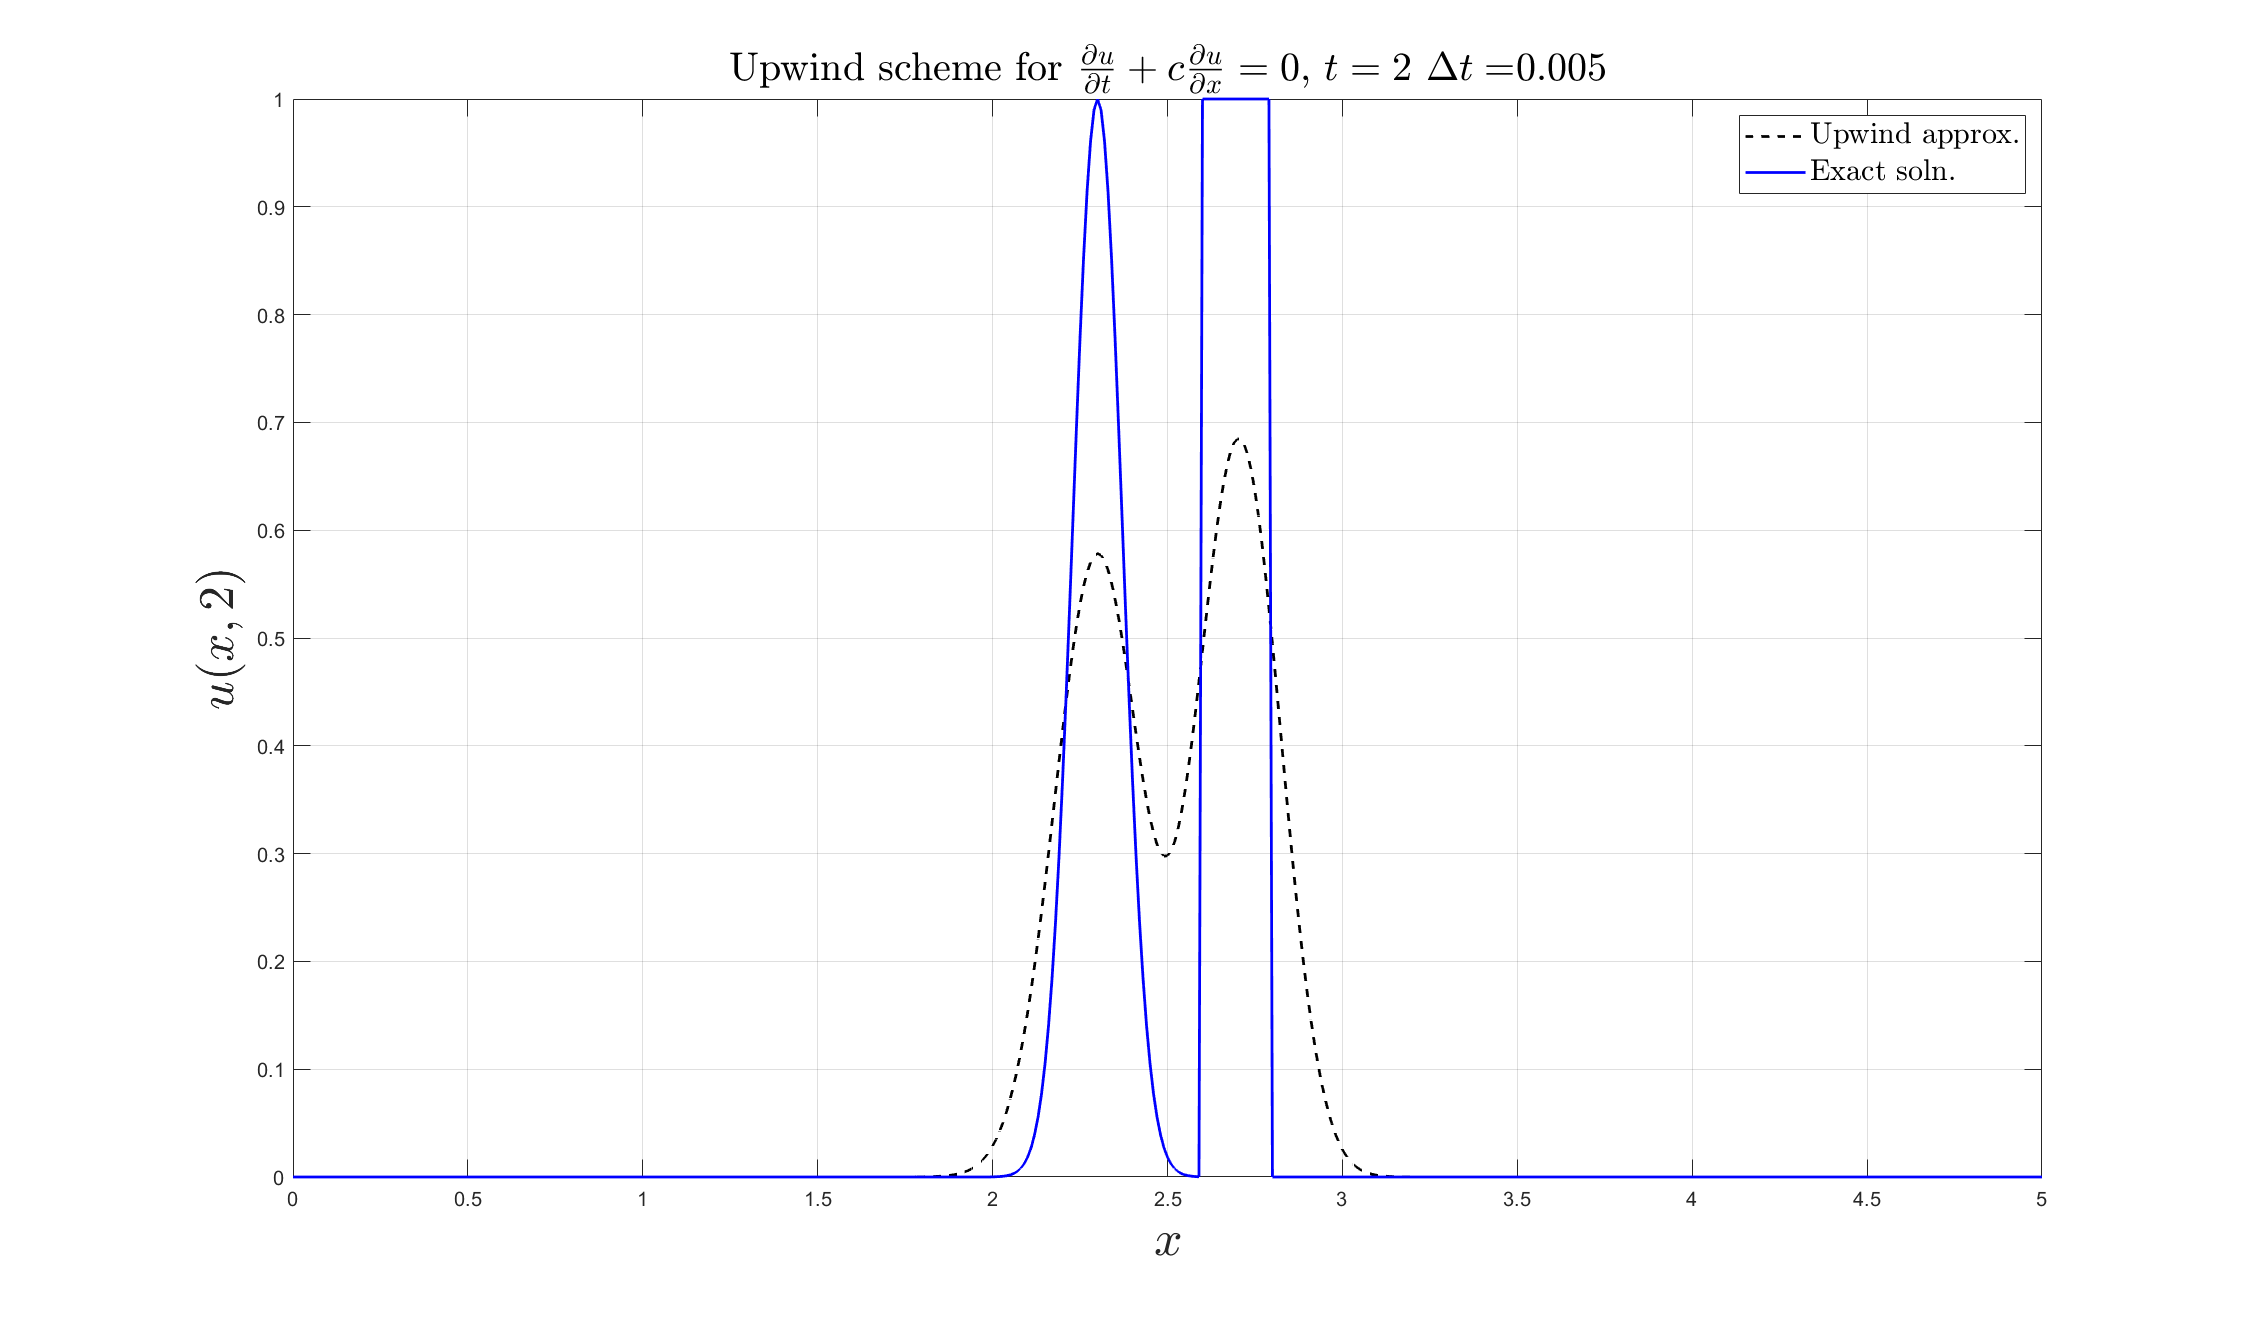
\includegraphics[scale = 0.25]{upwind_dt_005.png}
        \caption{$\ell^2$ error of approximately $2.8 \times 10^{-2}$}
    \end{figure}
    Note the high amount of diffusivity in the approximate solution; the square wave ``smoothed" out into a Gaussian and both the Gaussian and the square wave initial conditions displayed decay in their amplitudes. Further note that the upwind scheme preserved the speed of the waves. We note that this is very similar to the Upwind finite difference scheme for the 1D advection equation; the numerical solution advects at the prescribed speed, but we see a relatively high amount of diffusivity in the scheme. 

    Further, by setting $\Delta t = \Delta x$ (that is, $\nu = 1$), the diffusivity disappears and our numerical solution in visibly indistinguishable from the exact solution:
    \begin{figure}[H]
        \centering
        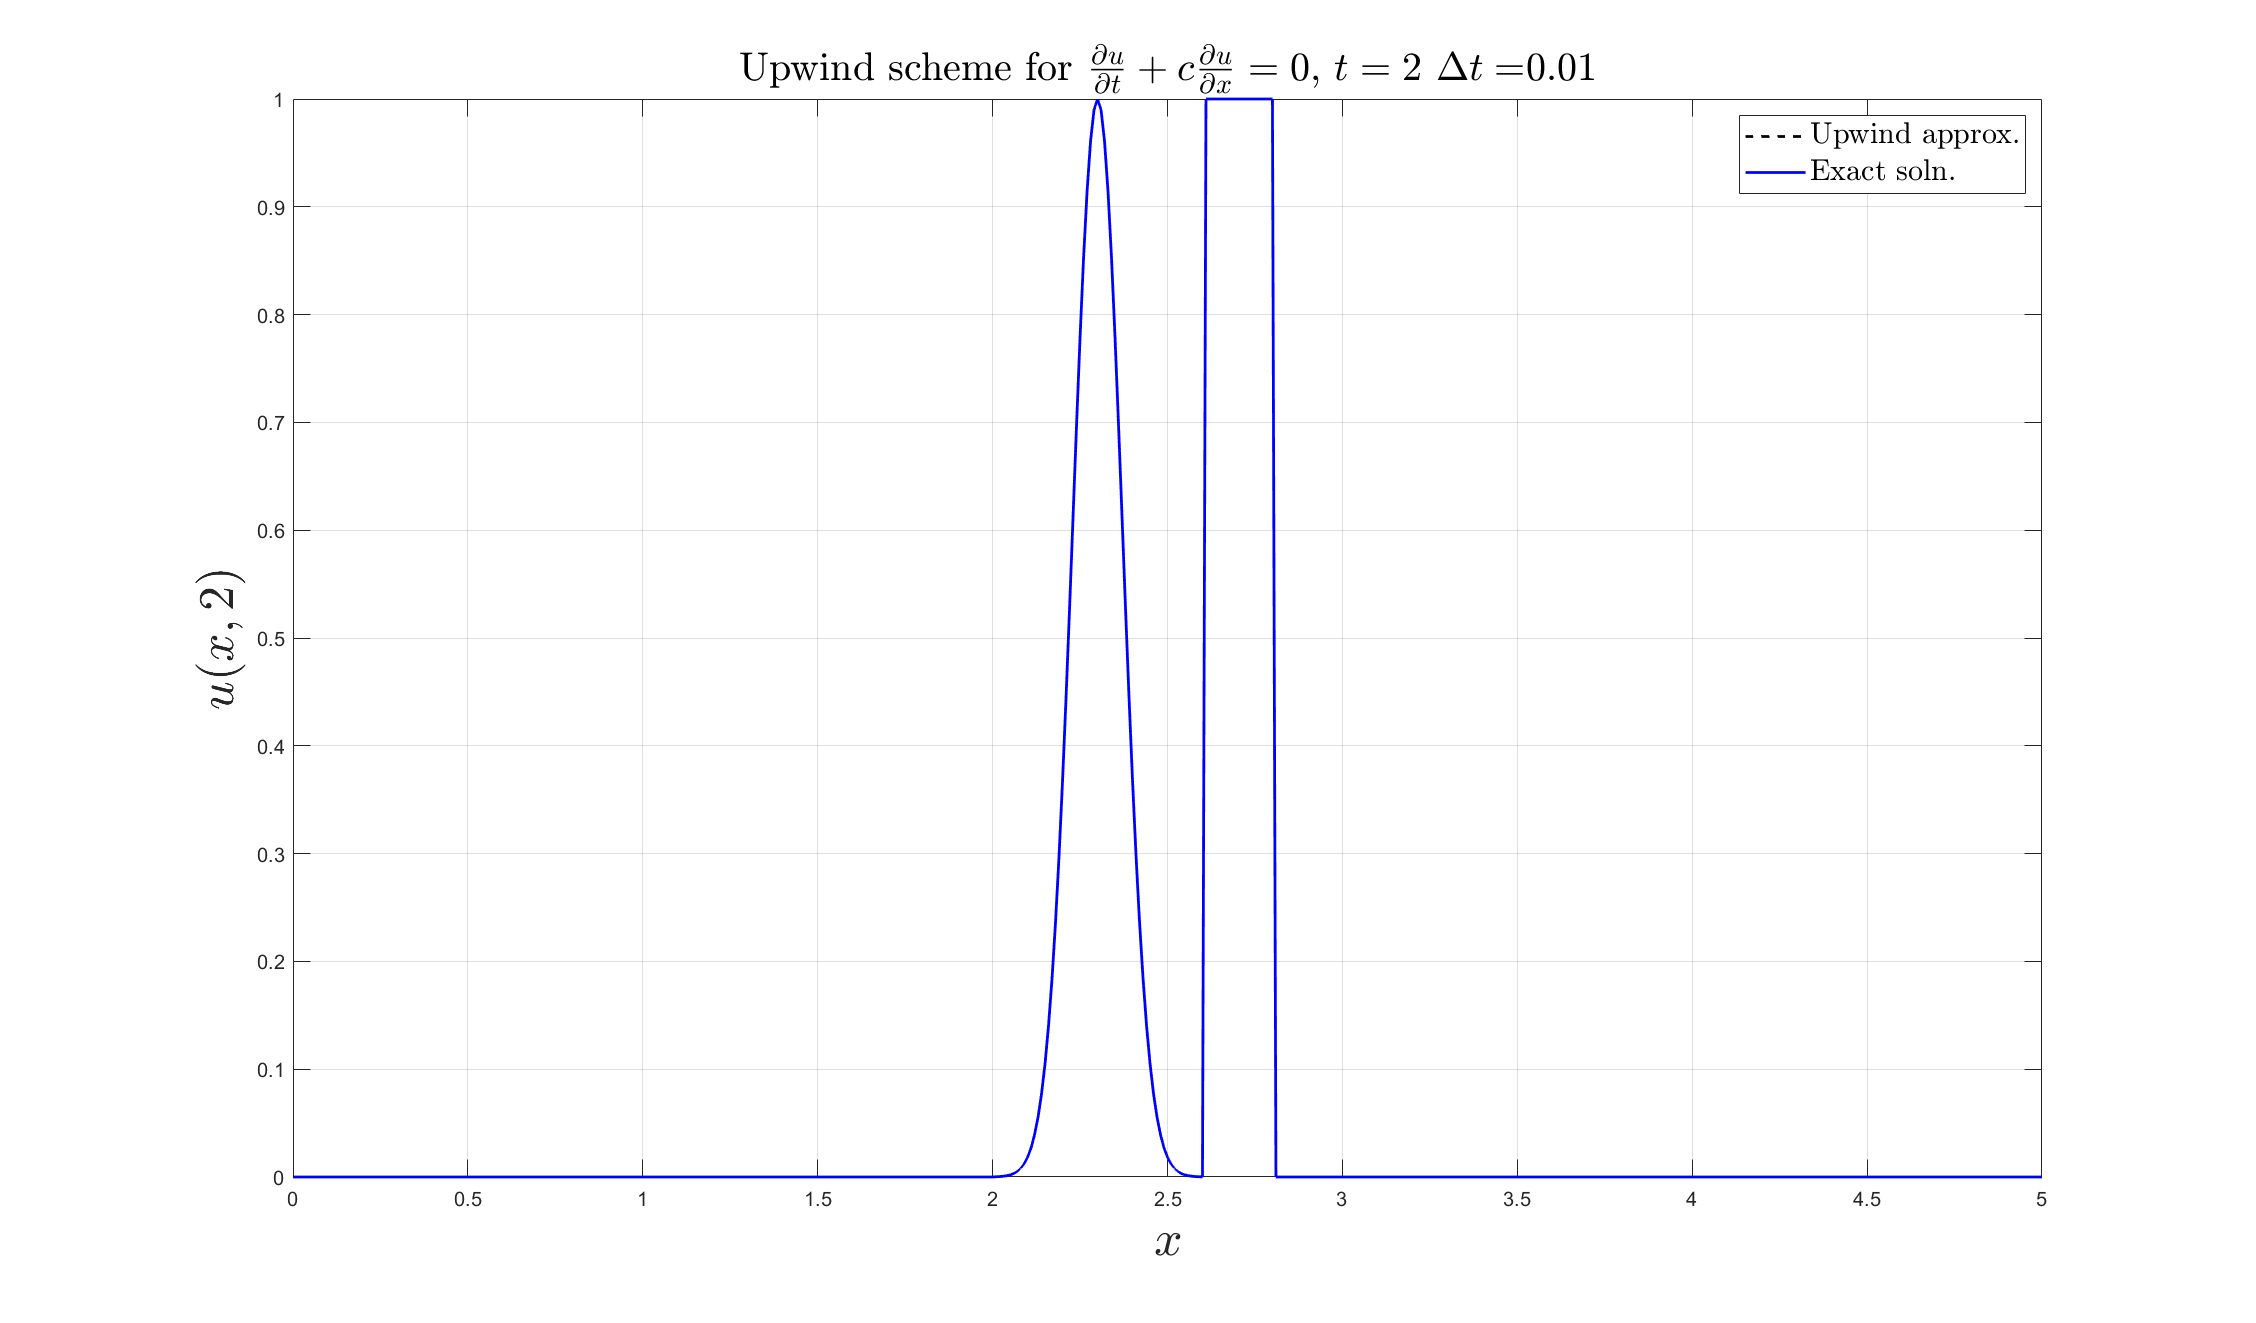
\includegraphics[scale = 0.25]{upwind_dt_001.png}
        \caption{$\ell^2$ error of approximately $4.4 \times 10^{-16}$, about twice double precision. Note how the exact and approximate solutions are virtually indistinguishable.}
    \end{figure}
    This is also the case for the Upwind scheme for finite differences; setting $\nu = 1$ causes the diffusivity to disappear. The reason for this is due to the fact that for the leading order terms in the modified equation for the Upwind f.d. scheme, a factor of $(\nu - 1)$ appears, so setting $\nu = 1$ cancels these terms out. Note that this is the case since for this implementation, the Upwind scheme is identitcal to the Upwind scheme for finite differences.

    
    \pagebreak
    \item[(2)] Minmode limit function
    \newline\newline

    \begin{figure}[H]
        \centering
        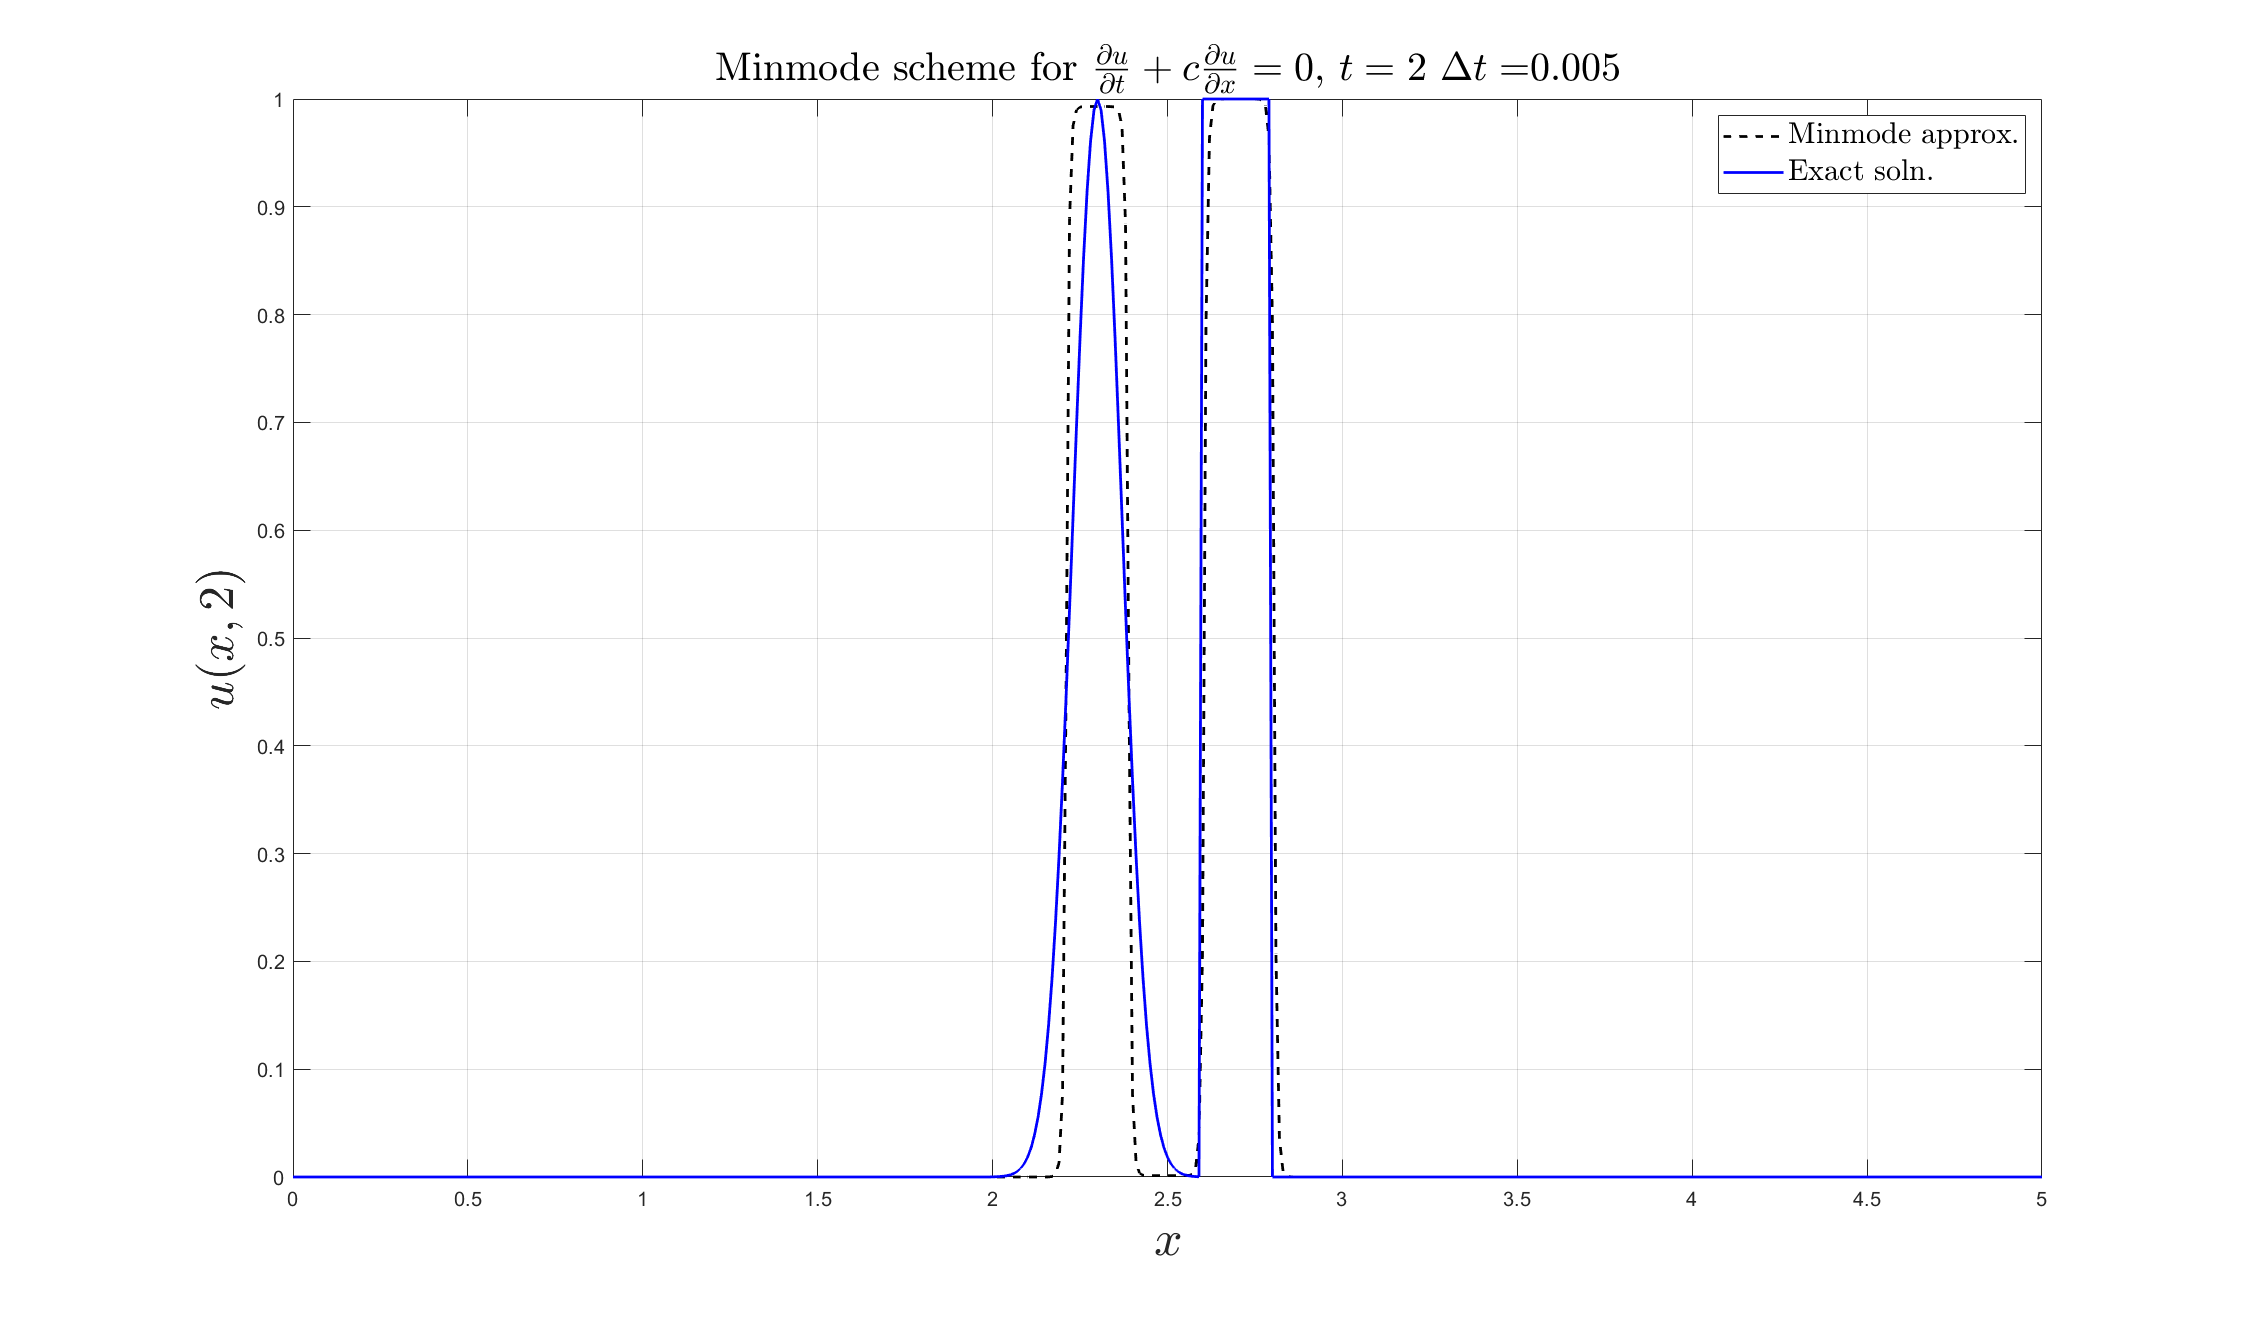
\includegraphics[scale = 0.25]{minmode_dt_005.png}
        \caption{$\ell^2$ error of approximately $1.6 \times 10^{-2}$. }
    \end{figure}
    With the Minmode limit function scheme, notice that the Gaussian gets a little squared off, the peak flattens out a little bit. The square wave is farily well approximated, with what appears to be a small amount of leading phase error.


    \pagebreak
    \item[(3)] Superbee limit function
    \newline\newline

    \begin{figure}[H]
        \centering
        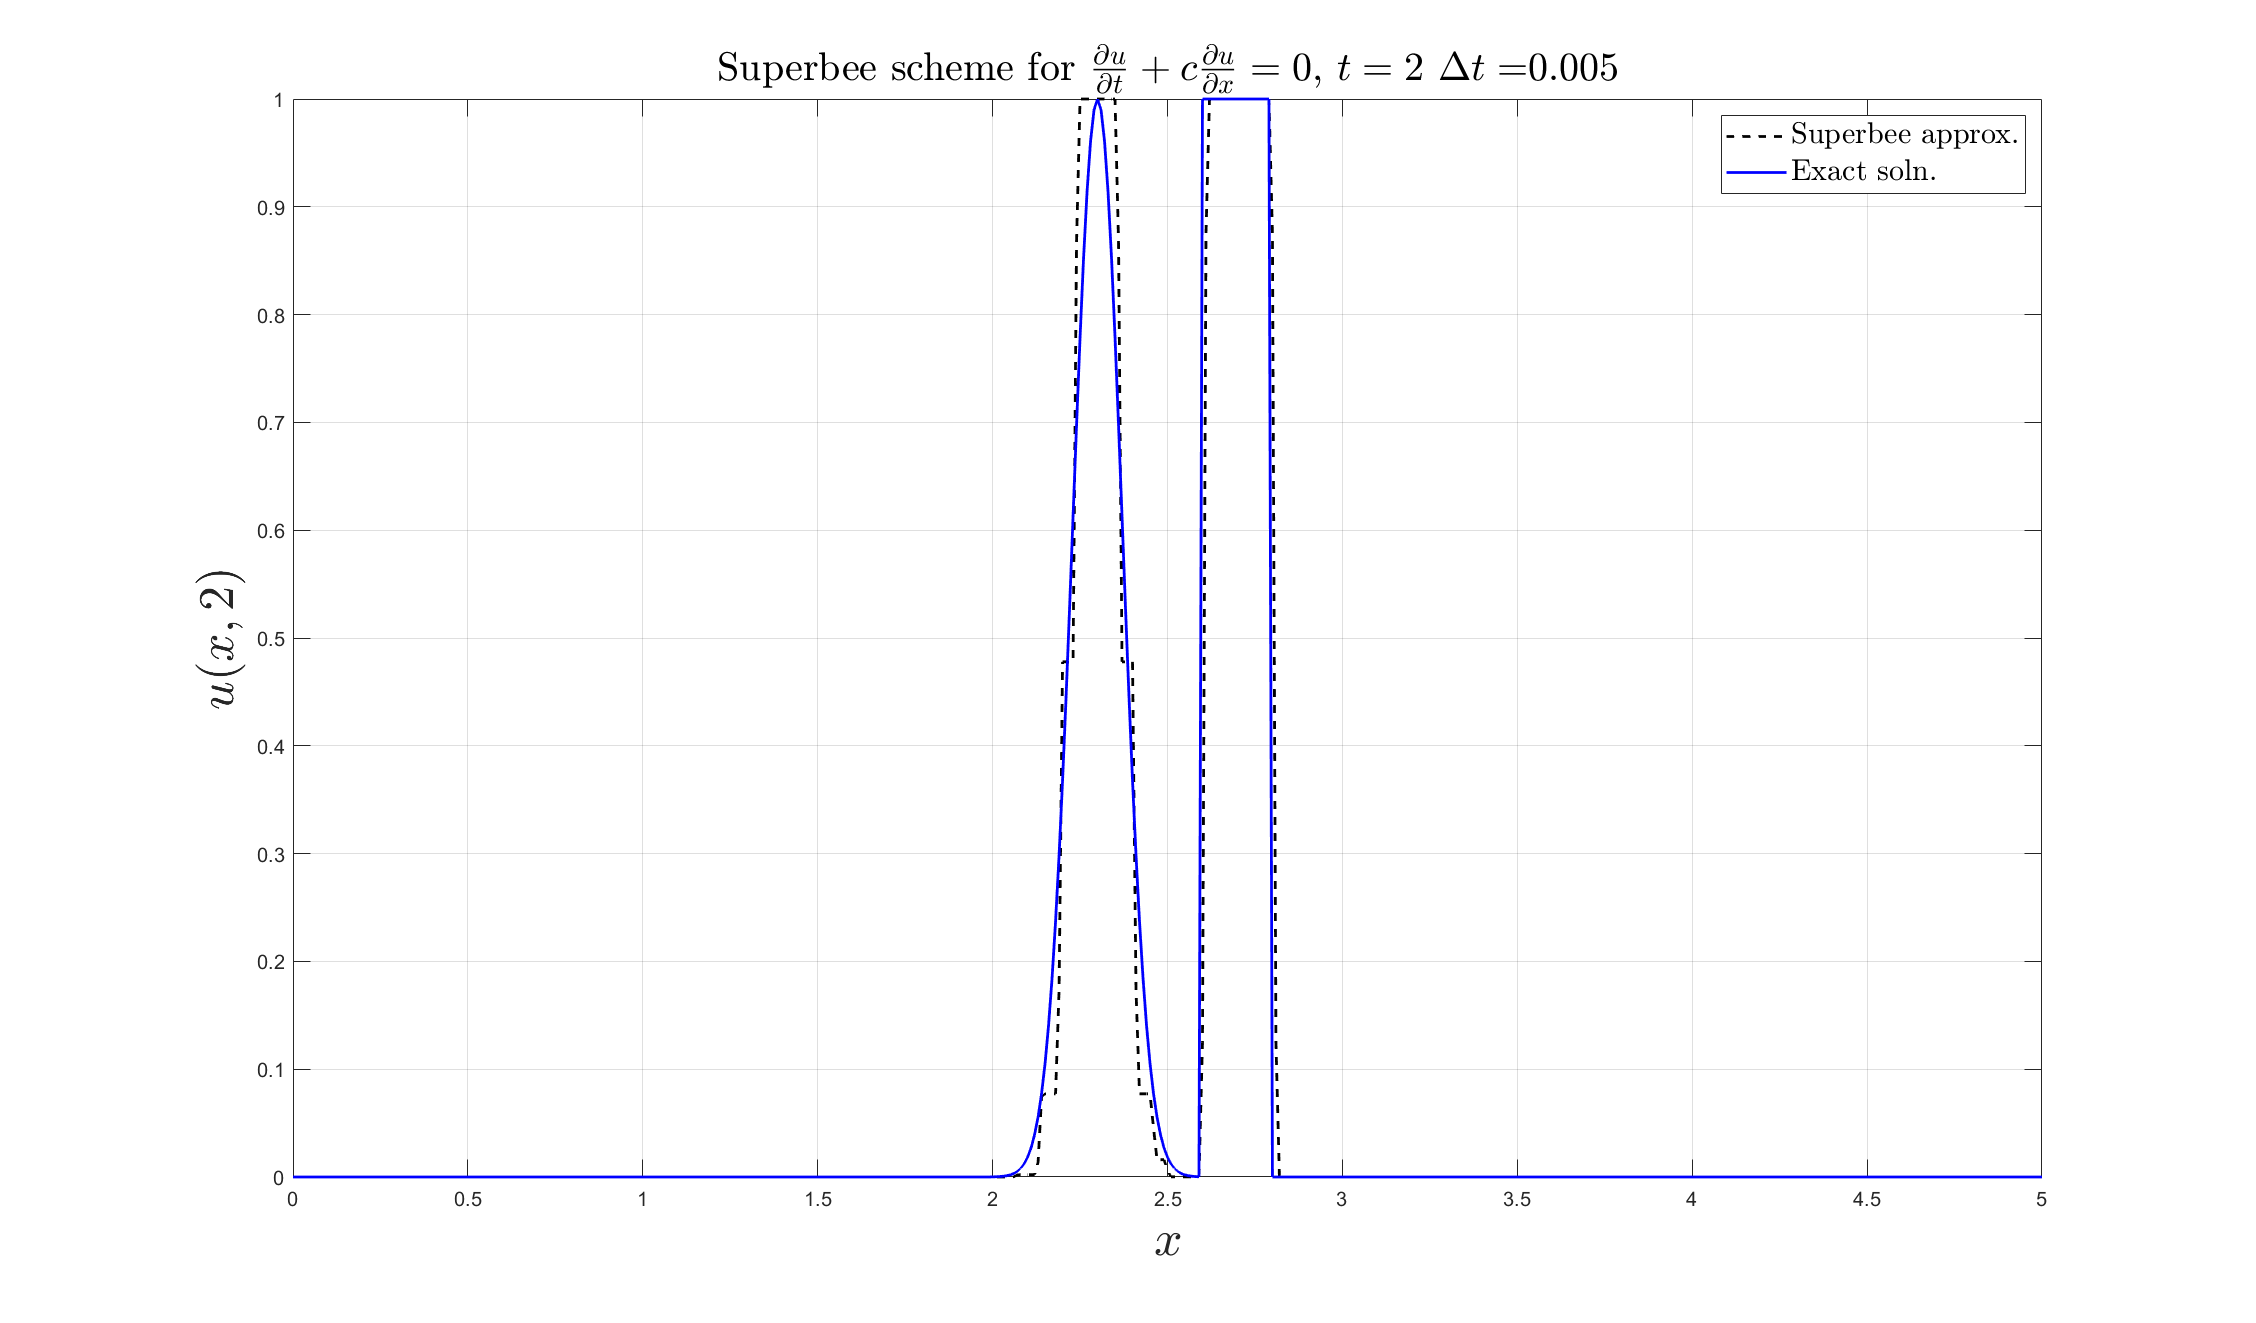
\includegraphics[scale = 0.25]{superbee_dt_005.png}
        \caption{$\ell^2$ error of approximately $1.4 \times 10^{-2}$}
    \end{figure}
    Similar to the minmode limiter function, we see what appears to be a minor amount of phase leading error in the square wave. Also observe that the Gaussian has been squared off with some ``stepping" in the shape.

    \pagebreak
    \item[(4)] Van Leer limit function
    \newline\newline

    \begin{figure}[H]
        \centering
        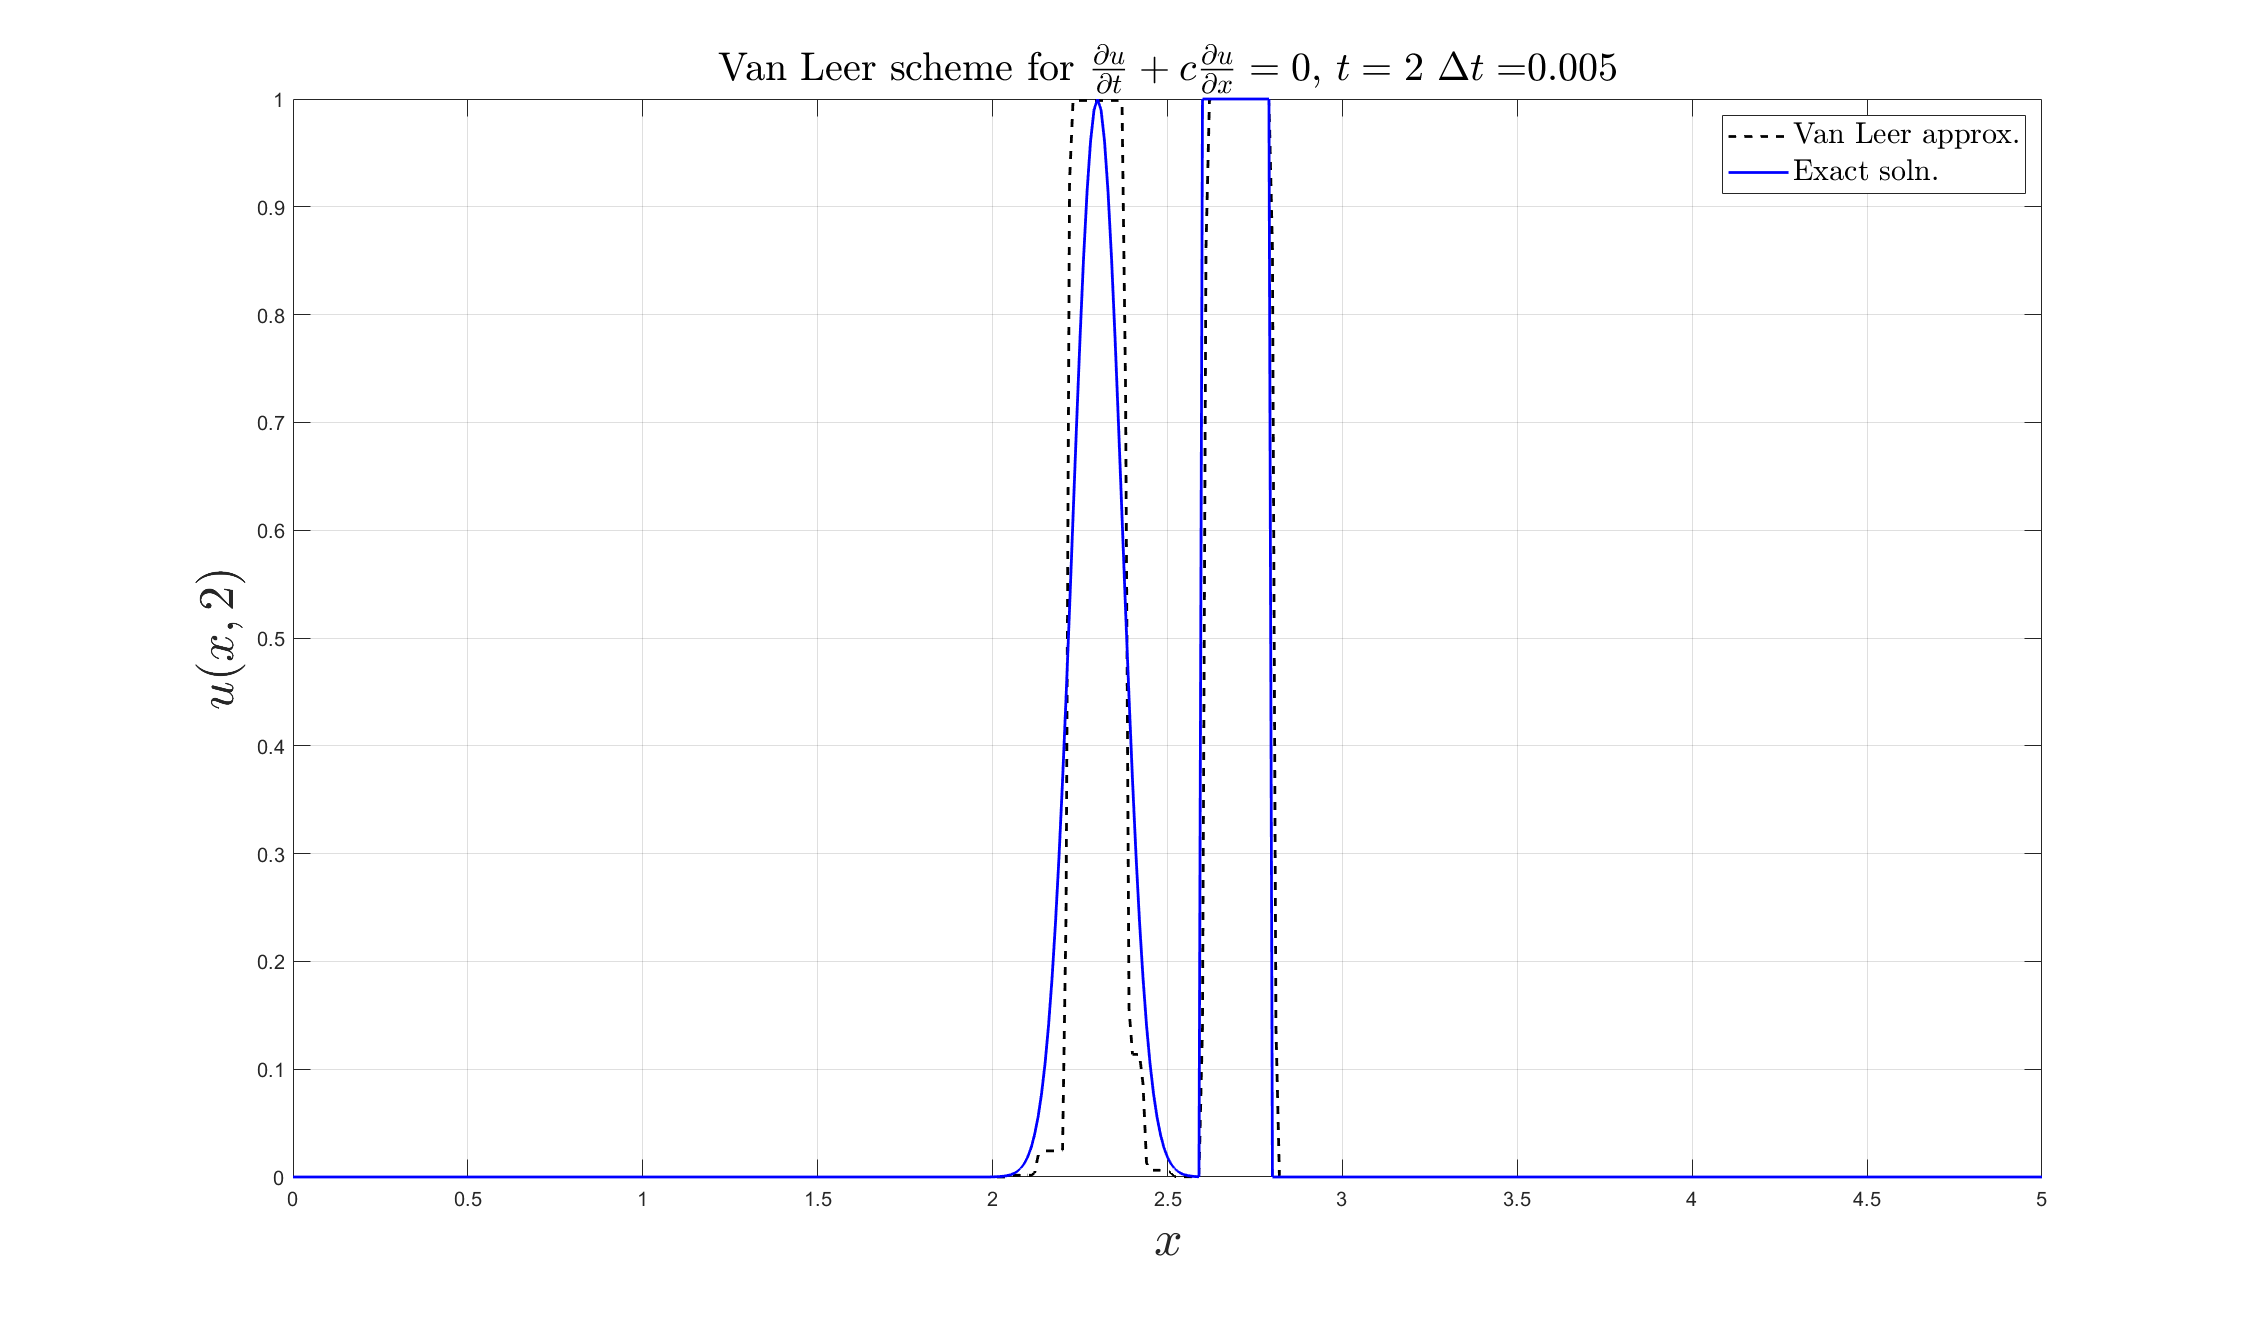
\includegraphics[scale = 0.25]{van_leer_dt_005.png}
        \caption{$\ell^2$ error of approximately $1.7 \times 10^{-2}$}
    \end{figure}
    Extremely similar results to the Suberbee limiter function.
\end{itemize}

\pagebreak
\section*{Discussion}
In this short project we implemented a finite element scheme utilizing the (1) Upwind (2) Minmode (3) Superbee (4) Van Leer limiter function scheme on the 1D advection equation $u_t + cu_x = 0$ with a Gaussian/square wave initial condition and $c = 1$. We took an equispaced discretization of the interval $[0,5]$ with $\Delta x = 0.01$ and ran the simulation from $t_0 = 0$ to $t_{\text{end}} = 2$ with a time step size of $0.005$.

    With these schemes and parameters, we observe some interesting numerical effects of the different schemes. Things to note are that each of the schemes appear to mostly preserve the wave speed $c = 1$. That is, we do not see any dispersive effects.  A note of interest is that the Upwind scheme (1) displayed a large amount of diffusive error, causing the amplitude of the numerical solution to decay over time. We also observe smoothing of the square wave initial condition; as the simulation progressed, the square wave smoothed out to become what appears to be a Gaussian. We further note that the Upwind scheme had the largest $\ell^2$ error of the four schemes studied.

    For the Minmode scheme (2), we see that the scheme did a good job at approximating the square wave initial condition, with a minor amount of smoothing around the discontinuities. Another thing of note is that the Gaussian became ``squared out". That is to say the peak got flattened out while the tails of the Gaussian straightened out. We also observe what appears to be a small amount of phase leading error in the square wave.

    In the Superbee scheme (3), we see similar results for the square wave as in the implementation of the Minmode scheme. That is, we observe what appears to be a small amount of leading phase error, with less smoothing near the discontinuities of the square wave. In contrast to the Minmode scheme, we observe some ``stairstepping". That is, the numerical approximation of the Gaussian becomes a step-like function that is symmetric over the axis of symmetry of the Gaussian.

    Finally, for the Van Leer (4) scheme, we observe very similar results as in the Superbee scheme. The numerical effects on the square wave are effectively the same as in (3), with similar results for the Gaussian. We still observe stairstepping for the numerical Gaussian, however, the numerical approximation is no longer symmetric and we observe slightly higher $\ell^2$ error when compared to (3).

    \pagebreak
    \section*{Code Snippet}
    \begin{lstlisting}[style = Matlab-editor]
        %FEM upwind
clear all; close all;

%spatial grid spacing
dx = 0.01;

%spatial grid endpoints
x0 = 0;
xend = 5;

%final time
tend = 4;

%x discretization
x = x0:dx:xend;

%number of spatial points
Nx = length(x);


%initially initialize initial condition 
u = zeros(length(x),1);

%temporal grid spacing
dt = dx/2;


method = 2;

%Limiter functions
switch method
    %Upwind scheme
    case 1
        psi = @(r) 0*r;
        methodStr = "Upwind";

    %Minmode scheme
    case 2
        psi = @(r) max(0,min(1,r));
        methodStr = "Minmode";

    %Superbee scheme
    case 3
        psi = @(r) max([0, min(2*r,1), min(r,2)]);
        methodStr = "Superbee";

    %Van Leer scheme
    case 4
        psi = @(r) (r + abs(r))./(1 + r);
        methodStr = "Van Leer";

    %QUICK scheme
    case 5
        psi = @(r) 1/4*(3 + r);
        methodStr = "QUICK";

    %MUSCL scheme
    case 6
        psi = @(r) max([0, min([2*r, (r+1)/2,2])]);
        methodStr = "MUSCL";
end


%wave speed
c = 1;

%exact solution (for Gaussian - need to add square wave)
% uEx = @(t) exp(-100*(x - 3/10 - c*t).^2);
uEx = zeros(length(x),1);

%build initial condition
for i = 1:length(x)
    if (0 <= x(i) && x(i) <= 0.6)
       u(i) = exp(-100*(x(i) - 0.3).^2);

    elseif (0.6 < x(i) && x(i) <= 0.8)
        u(i) = 1;
    end
end


%courant number or something or other
nu = c*dt/dx;

%enforce left BC
u(1) = 0;

%t0 for keeping track of time for exact solution
t0 = 0;

%number of time steps
Nt = tend/dt;


%include in denominator to avoid division by 0
eps = 1e-10;

%initialize placeholder for updating the approximate solution
unew = zeros(size(u));

%time stepping
for j=1:Nt
    t0 = t0 + dt;
    %minmode limiter function
    for i = 3:Nx-1
        
        %r at the east edge
        re = (u(i) - u(i-1))/(u(i+1) - u(i) + eps);
        psi_e = psi(re);

        %r at the west edge
        rw = (u(i-1) - u(i-2))/(u(i) - u(i-1) + eps);
        psi_w = psi(rw);


        ue = u(i) + 1/2*psi_e*(u(i+1) - u(i));

        uw = u(i-1) + 1/2*psi_w*(u(i) - u(i-1));

        %update step
        unew(i) = u(i) - nu*(ue - uw);
        % unew(i) = u(i) - nu*(u(i) + psi_e*(u(i+1) - u(i)) - u(i-1) - psi_w*(u(i) - u(i-1)));

    end

    %enforce boundary conditions
    unew(1) = 0;
    unew(2) = 0;
    % unew(end) = 0;
    
    %update u
    u = unew;

    uEx = zeros(size(x));

    % %update exact solution
    % for k = 1:length(x)
    %     if (c*t0 <= x(k) && x(k) <= 0.6 + c*t0)
    %        uEx(k) = exp(-100*(x(k) - 0.3 - c*t0).^2);
    % 
    %     elseif (0.6 + c*t0 < x(k) && x(k) <= 0.8 + c*t0)
    %         uEx(k) = 1;
    %     end
    % end
    % 
    % %plot the approximate solution at each time step
    % plot(x,u, 'k--', x, uEx, 'b-', 'linewidth', 1.4)
    % xlabel('$x$', 'fontsize', 25, 'interpreter', 'latex')
    % ylabel('$u(x,2)$', 'fontsize', 25, 'interpreter', 'latex')
    % title(methodStr + " scheme for $\frac{\partial u}{\partial t} + c\frac{\partial u}{\partial x} = 0$, $t = 2$" + " $\Delta t = $" + num2str(dt), 'fontsize', 20, 'interpreter', 'latex')
    % legend(methodStr + " approx.", "Exact soln.", 'fontsize', 15, 'interpreter', 'latex')
    % grid on
    % drawnow
  
end

for k = 1:length(x)
        if (c*t0 <= x(k) && x(k) <= 0.6 + c*t0)
           uEx(k) = exp(-100*(x(k) - 0.3 - c*t0).^2);
    
        elseif (0.6 + c*t0 < x(k) && x(k) <= 0.8 + c*t0)
            uEx(k) = 1;
        end
end

plot(x, u, 'k--', x, uEx, 'b-', 'linewidth',1.4)
xlabel('$x$', 'fontsize', 25, 'interpreter', 'latex')
ylabel('$u(x,2)$', 'fontsize', 25, 'interpreter', 'latex')
title(methodStr + " scheme for $\frac{\partial u}{\partial t} + c\frac{\partial u}{\partial x} = 0$, $t = 2$" + " $\Delta t = $" + num2str(dt), 'fontsize', 20, 'interpreter', 'latex')
legend(methodStr + " approx.", "Exact soln.", 'fontsize', 15, 'interpreter', 'latex')
grid on
axis tight

err = dx*norm(u - uEx.',2)
    \end{lstlisting}
\end{document}
